\chapter{Filtrage}
\label{chap:filtrage}
	Un filtre est un dispositif visant à modifier le contenu fréquentiel d'un signal. Une utilisation courante est de supprimer d'un signal des composantes fréquentielles indésirables (ou, inversement, d'extraire de ce signal certaines composantes utiles). La figure \ref{Fig:Effet_filtre_bruit} illustre ce type d'utilisation. Le graphique à gauche présente un signal digital corrompu par un bruit aléatoire important. La présence de ce bruit est indésirable, car il risque de corrompre l'interprétation de ce signal. Afin d'éviter toute erreur de décodage de ce signal, un filtre doit être synthétisé pour supprimer ce bruit, sans trop affecter le signal utile. L'utilisation d'un filtre est possible si le signal utile et le bruit occupent des bandes de fréquence différentes. Un outil d'analyse du signal, comme la transformée de Fourier que nous aborderons dans le prochain chapitre, permet de déterminer l'occupation fréquentielle des signaux.
	
	Dans l'exemple ci-dessous, le signal utile à une fréquence de 2.5 Hz. Le spectre du signal bruité est présenté à la figure \ref{Fig:Effet_filtre_bruit_spectre}. Le spectre du signal utile se situe principalement en dessous de 100 Hz. Le bruit est large bande, mais présente quatre composantes spectrales importantes au-dessus de 100 Hz. Pour éliminer ce bruit, on dimensionne un filtre passe-bas d'ordre 2 avec une fréquence de coupure de 100 Hz. L'effet de ce filtre sur le signal est présenté sur la partie droite de la figure \ref{Fig:Effet_filtre_bruit}. La présence du bruit n'est quasiment plus discernable. Comme le confirme le spectre du signal filtré (\ref{Fig:Effet_filtre_bruit_spectre}), le filtre a fortement atténué le spectre au-dessus de 100 Hz. On peut remarquer que le filtre affecte aussi la forme du signal utile, mais cet effet reste négligeable et ne contribuera pas à une erreur d'interprétation du signal.  
	
	\begin{figure}[h]
		\centering
		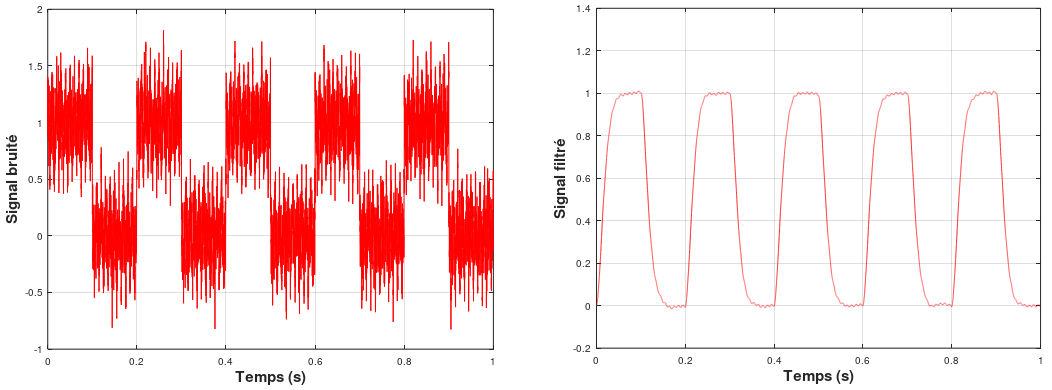
\includegraphics[scale=0.6]{images/Effet_filtre_bruit.png}
		\caption{Effet du filtre sur un signal bruité : signal bruite (à gauche) et filtré (à droite)}	
		\label{Fig:Effet_filtre_bruit} 
	\end{figure}

	\begin{figure}[h]
		\centering
		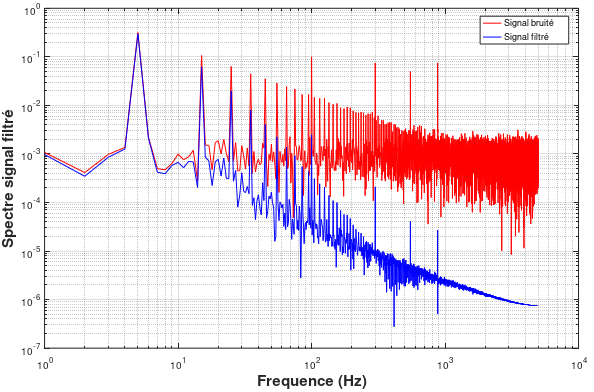
\includegraphics[scale=0.6]{images/Effet_filtre_bruit_spectre.png}
		\caption{Spectre du signal bruité et filtré}	
		\label{Fig:Effet_filtre_bruit_spectre} 
	\end{figure}
	
	
	Ce chapitre est dédié au filtre linéaire à temps invariant et leur analyse en régime harmonique. Les filtres n'ont aucune différence par rapport aux systèmes LTI vues précédemment. La différence vient de leur utilisation, qui nécessite une analyse dans le domaine fréquentiel. La connaissance de la fonction de transfert du filtre est donc centrale. En régime harmonique, nous la noterons H($\omega$) ou H(f).
	
	Dans ce chapitre, nous présenterons les outils et les termes usuels permettant de caractériser les filtres. Nous introduirons un outil d'analyse graphique : le diagramme de Bode et son tracé asymptotique.  
	

	
	\section{Définition d'un filtre}
	
	\subsection{Définition}
	
	Un filtre est un système, généralement passif, présentant une certaine sélectivité dans le domaine des fréquences. Il est utilisé pour atténuer (ou au contraire laisser passer) le signal sur une ou plusieurs bandes de fréquences.
	Il atténue ainsi certaines des composantes fréquentielles du signal d’entrée et en laisse passer d’autres, d’où son appellation de filtre ! C’est bien cette opération sélective d’atténuation ou d’amplification des fréquences que modélise la multiplication de l'excitation par la fonction de transfert.
	\begin{equation}\label{}
	Y(f) = H(f) \cdot X(f)
	\end{equation}

	Une manière pratique d'étudier un filtre est de l'analyser en régime harmonique, donc dans le domaine fréquentiel. Pour mettre en évidence l'effet du filtre, la fonction de transfert peut être écrite sous la forme module-argument :
	
	\begin{equation}\label{key}
	H(f) = |H(f)|exp(j~arg(H(f)))
	\end{equation}
	
	 Le module correspond au gain du filtre, c'est-à-dire le rapport entre les amplitudes de la réponse du filtre et de son excitation. Si le module est important, alors le signal d'entrée est faiblement atténué voire amplifié. Sinon, il est filtré.
	Si les signaux d'entrée et de sortie représentent le même type de grandeur (par exemple, une tension dans le cas de signaux électriques), le gain est sans unité.\\ 
	
	L'argument correspond au déphasage apporté par le filtre. Celui-ci traduit un retard $ \tau $ introduit par le filtre à la fréquence f, déterminé par l'équation \ref{retard}.	
	
	\begin{equation}\label{retard}
	\tau = \frac{d(Arg(H(f)))}{2\pi df}
	\end{equation}
	
	\vspace{1\baselineskip}
	
	\underline{\textbf{Filtre à phase linéaire}}
	
	On remarque une propriété intéressante : soit un signal constitué de la superposition de plusieurs signaux sinusoïdaux, traverante un filtre présentant un déphasage variable en fonction de la fréquence. Même si le gain est le même à ces différentes fréquences, si le retard introduit par le filtre varie avec la fréquence, alors le signal en sortie présentera une distorsion. Ceci démontre qu'il ne faut pas négliger l'information de phase d'un filtre.
	Pour éviter cette distorsion, il est nécessaire que le retard soit constant. D'après \ref{retard}, cela est vérifié uniquement si le déphasage varie linéairement avec la fréquence. On parle alors de filtres à phase linéaire.
	
	On peut aussi remarquer qu'un filtre présentant un déphasage constant quelle que soit la fréquence ne doit pas être réalisable en pratique. En effet, celui-ci ne présenterait aucun retard. La sortie changerait simultanément avec l'entrée, ce qui est physiquement impossible.
	
	\vspace{1\baselineskip}
	
	\subsection{Filtre à réponse impulsionnelle réelle}
	Considérons le cas particulier, mais pratique, où la réponse impulsionnelle est une fonction réelle : $ \forall t \in \mathbb{R},~h(t) \in \mathbb{R}$. Une réponse temporelle prenant des valeurs complexes n’aurait pas directement de sens physique ! On peut alors appliquer la propriété suivante de la Transformée de Fourier : la Transformée de Fourier d’une fonction réelle est une fonction en général complexe mais admettant une symétrie conjuguée : $\forall f \in \mathbb{R},~H^{*}(f) = H(-f)$, c'est-à-dire dont le module est une fonction paire tandis que l’argument est une fonction impaire, comme le montre l'équation ci-dessous. 
	
	\begin{equation}\label{key}
	\forall f \in \mathbb{R},~|H(f)| = |H(-f)| ~~et~~arg(H(f)) = -arg(H(-f))
	\end{equation}
	
	\begin{figure}[h]
		\centering
		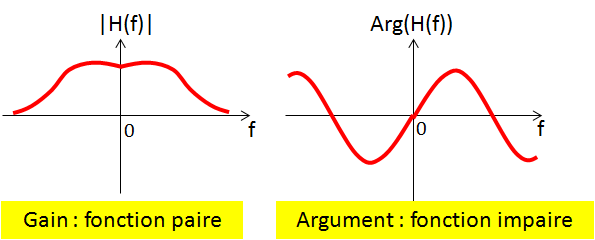
\includegraphics[scale=0.6]{images/symetrie_filtre_reel.png}
		\caption{Symétries du module et de l'argument d'un filtre réel}	
		\label{Fig:symetrie_filtre_reel} 
	\end{figure}
	 
	
	\subsection{Fréquence négative}
	
	Comme nous l'avons vu dans les chapitres précédents, la fréquence est une grandeur réelle pouvant être négative. En raison de propriétés de symétries introduites par la transformée de Fourier pour les fonctions réelles, les représentations que nous utiliserons dans ce chapitre ne font apparaître que les fréquences positives. Les fréquences négatives sont omises par convention parce qu'elles n'apportent pas d'informations supplémentaires : le gain est une fonction paire tandis que le déphasage est une fonction impaire.
	
	La notion de basse ou de haute fréquence ne s’attache qu’à la valeur absolue de la fréquence considérée : seules les fréquences positives f appartenant à $\mathbb{R}^{+}$ ont un sens physique ; les fréquences négatives f appartenant à $\mathbb{R}^{-}$ n’ont pas de signification physique directe, mais leur prise en compte assure une utilisation correcte de l’analyse harmonique comme outil d’étude des filtres.
	
	Ainsi, la convention pratique veut que le tracé des caractéristiques des gains et déphasage des filtres (diagramme de Bode), la définition des fréquences de coupure et des bandes passantes soient uniquement donnés dans le domaine des fréquences positives. Ils existent aussi pour les fréquences négatives, mais sont obtenus facilement par symétrie.
	
	\vspace{1\baselineskip}
	
	\section{Analyse harmonique}
	A partir de la connaissance du gain et du déphasage de la fonction de transfert, lorsque le filtre est attaqué par un signal (co)sinusïdal, il est très simple de déterminer l'expression de sa réponse. En considérant une notation complexe, la réponse temporelle du filtre en régime harmonique est donnée par :
	\begin{equation}\label{}
	x(t) = Re[X_{0}exp(j\Phi_{x})exp(j2\pi ft)] \Rightarrow y(t) = Re[X_{0}|H(f)exp(j(\Phi_{x}+arg(H(f))))exp(j2\pi ft)]
	\end{equation}
	Celle-ci peut aussi s'écrire sous la forme suivante :
	\begin{equation}\label{key}
	x(t) = X_{0}cos(2\pi ft+\Phi_{x}) \Rightarrow y(t) = X_{0}|H(f)+cos(2\pi ft+\Phi_{x}+arg(H(f)))
	\end{equation}
	
	\section{Représentation - Diagramme de Bode}
	\subsection{Diagramme de Bode}
	En régime harmonique, l'étude d'un filtre passe par une analyse de son gain et de son déphasage. Il faut donc chercher une représentation graphique adaptée à l'analyse du comportement fréquentiel du filtre. La méthode la plus courante est le tracé du diagramme de Bode. Il contient deux tracés graphiques décrivant :
	\begin{itemize}
		\item l'évolution du gain en fonction de la fréquence
		\item l'évolution du déphasage en fonction de la fréquence
	\end{itemize}

	\vspace{0.5\baselineskip}

	Bien qu'il n'existe pas une forme de représentation unique du diagramme de Bode, certains usages sont récurrents et il convient de les expliquer. Pour des raisons pratiques, l'axe fréquentiel est généralement tracé en échelle logarithmique. En général, on s'intéresse au comportement fréquentiel sur une large gamme de fréquence, couvrant plusieurs décades. Un tracé avec une échelle linéaire offre une résolution constante, qui cache les détails dans les basses fréquences. Avec un tracé en échelle logarithmique, la résolution varie en fonction de la fréquence et s'adapte à chaque décade. Le même niveau de détail peut être apprécié en basse ou en haute fréquence. C'est ce qu'illustre la figure \ref{Fig:Effet_Flin_log} : le filtre étudié est de type passe-bas, c'est-à-dire qu'il laisse passer les signaux basses fréquences. Le tracé est réalisé entre 100 Hz et 1 MHz. Avec l'échelle linéaire, le tracé ne permet pas d'évaluer précisément à partir de quelle fréquence le filtre commence à atténuer significativement le signal d'entrée. Avec l'échelle logarithmique, on peut mieux évaluer cette fréquence, appelée fréquence de coupure, qui se situe aux alentours de 1 kHz.
	\begin{figure}[h]
		\centering
		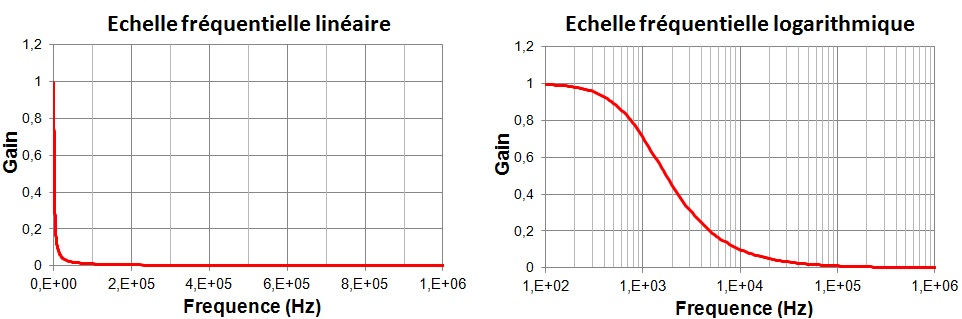
\includegraphics[scale=0.6]{images/Effet_Flin_log.jpg}
		\caption{Tracé du gain de la fonction de transfert d'un filtre passe-bas : échelle fréquentielle linéaire (à gauche) et logarithmique (à droite)}	
		\label{Fig:Effet_Flin_log} 
	\end{figure}
	
	\textbf{\underline{Conseil pratique : comment tracer une échelle logarithmique ?}}
	
	On définit tout d'abord le pas représentant une décade (par exemple 2 cm par décade). On considère que l'origine est placé en f=1 (log10(1) = 0). La position de toute valeur par rapport à cette origine sera donnée par pas $\times log_{10}(valeur)$. Ainsi, la valeur 10 (une décade de plus que 1) sera située à 2 cm à droite de l'origine, 100 (deux décades de plus) sera située à 4 cm à droite de l'origine, tandis que 0.1 (une décade de moins) sera située à 2 cm à gauche de l'origine. Par exemple, la valeur 50 sera située à $2\times log10(50)$ = 3.4 cm à droite de l'origine.\\
	
	Une autre convention consiste à exprimer les gains en décibels (\ref{dB}), qui n'est rien d'autre qu'une représentation des valeurs sur une échelle logarithmique. De part leur sélectivité en fréquence, les gains des filtres vont présenter des valeurs très variables en fonction de la fréquence. Pour les mêmes raisons que la représentation des fréquences, une échelle logarithmique pour le gain permettra d'apprécier avec la même résolution les faibles et les fortes valeurs de gain. La figure \ref{Fig:Effet_Ylin_dB} l'illustre, en reprenant l'exemple du tracé du gain du filtre précédent. Le tracé du gain sur une échelle linéaire ne permet pas de le mesurer précisément lorsqu'il atteint de faibles valeurs. A contrario, lorsqu'il est exprimé en dB, la mesure des faibles valeurs devient plus précise, mettant en évidence les tendances particulières du gain. Par exemple, le gain de ce filtre décroit avec une pente de -20 dB par décade au-dessus de la fréquence de coupure, ce qui est typique d'un filtre passe-bas d'ordre 1. 
	\begin{equation}\label{dB}
	G_{dB} = 20 \cdot log(|H(f)|)
	\end{equation}
	
	\begin{figure}[h!]
		\centering
		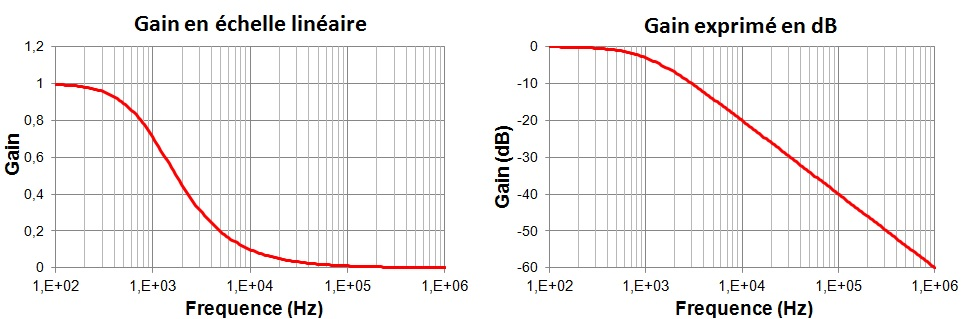
\includegraphics[scale=0.6]{images/Effet_Ylin_dB.jpg}
		\caption{Tracé du gain de la fonction de transfert d'un filtre passe-bas : échelle linéaire (à gauche) et en décibel (à droite)}	
		\label{Fig:Effet_Ylin_dB} 
	\end{figure}
	
	\begin{minipage}[l]{0.4\linewidth}
		Il n'y a pas de convention particulière pour le déphasage, qui peut être exprimé en radians ou en degrés. La figure ci-contre présente le diagramme de Bode du filtre précédent, montrant les tracés de l'évolution fréquentielle de son gain et de son déphasage. Le diagramme de Bode indique un déphasage dont la valeur diminue entre 0 et $-\frac{\pi}{2}$. Le déphasage étant négatif, le filtre introduit un retard.	
	\end{minipage} \hfill
	\begin{minipage}[c]{0.50\linewidth}
			%\centering
			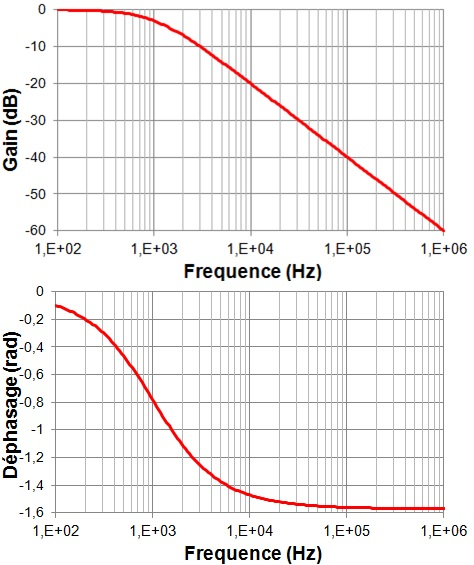
\includegraphics[scale=0.6]{images/Bode_passe-bas.jpg}
			%\caption{Diagramme de Bode d'un filtre passe-bas}	
			%\label{Fig:Bode_passe-bas} 	
	\end{minipage}

	\vspace{1\baselineskip}

		\textbf{\underline{Remarque : normalisation des fréquences :}}
	
	Un filtre de nature donnée présentera toujours la même tendance fréquentielle. Seule la ou les fréquences de coupure changeront selon les propriétés du filtre. Pour disposer d'une représentation indépendante de la fréquence de coupure, il est courant de représenter l'axe des fréquences sous la forme d'une fréquence normalisée. Cette normalisation se fait par rapport à une fréquence de référence, généralement la fréquence coupure du filtre. Ainsi, le même gabarit peut être utilisé pour plusieurs filtres présentant différentes fréquences de coupure. Si l'axe fréquentiel est exprimé en pulsation, la normalisation se fera de la même manière.
	\begin{equation}\label{key}
	f_{norm} = \frac{f}{f_{c}}
	\end{equation}
	\begin{equation}\label{key}
	\omega_{norm} = \frac{\omega}{\omega_{c}}
	\end{equation}
	
	\begin{figure}[h!]
		\centering
		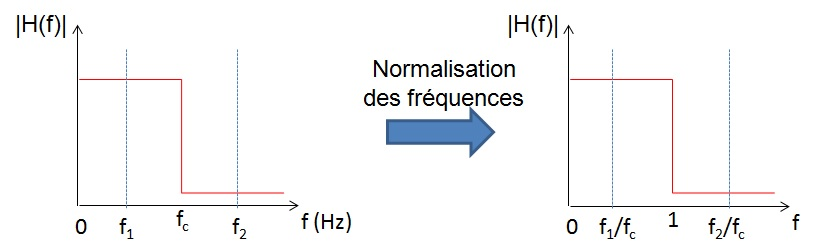
\includegraphics[scale=0.6]{images/freq_norm.jpg}
		\caption{Normalisation des fréquences}	
		\label{Fig:freq_norm} 
	\end{figure}
	

	
	
	\subsection{Tracé asymptotique du diagramme de Bode}
	
	Les fonctions de transfert des filtre linéaires peuvent souvent être écrites sous la forme d'un rapport de deux polynômes, comme le montre l'équation \ref{TF_usuelle_filtre}. Comme nous allons le voir, cette forme particulière facilite le tracé graphique du module de la fonction de transfert, sous une forme appelée tracé asymptotique. Celui-ci permet de visualiser ou représenter sans calculs compliqués l'évolution du module, les pentes, les points d'inflexion (fréquences de coupure) ou l'ordre du filtre. Il s'agit d'un outil d'ingénierie couramment utilisé, soit dans la synthèse de filtre comme moyen de définir le gabarit d'un filtre, ou bien de son analyse à partir de l'expression de sa fonction de transfert. 
	\begin{equation}\label{TF_usuelle_filtre}
	H(\omega)=G\frac{\prod_{i=1}^{m}(1+j\frac{\omega}{\omega_{i}})}{\prod_{j=1}^{n}(1+j\frac{\omega}{\omega_{j}})}
	\end{equation}
	
	Le tracé asymptotique est une représentation simplifiée du module, même s'il peut s'étendre à celui de la phase. Il consiste à représenter le comportement asymptotique de chacun des termes des produits au numérateur et au dénominateur de l'équation \ref{TF_usuelle_filtre}, où G est une constante réelle, $\omega_{i}$ représente les zéros et $\omega_{j}$ les pôles de la fonction de transfert. La représentation se fait systématiquement sur un graphique aux échelles log-log, avec l'utilisation de décibels sur l'axe des ordonnées. De cette manière, les termes de l'équation \ref{TF_usuelle_filtre} présenteront des décroissances linéaires en +/- 20 dB/dec. En outre, les produits et les divisions se transformeront en addition ou en soustraction, opérations plus simples (on rappelle que $log(a \cdot b)=log(a)+log(b)$ et log($\frac{a}{b})=log(a)-log(b)$).
	
	Nous allons illustrer le tracé asymptotique du module et de la phase d'une fonction de transfert quelconque. Mais avant, nous allons réaliser ceux des termes de base de l'équation \ref{TF_usuelle_filtre}. Dans les différents exemples, nous allons considérer une pulsation de coupure $\omega_{i} = 100~rad/s$. Commençons par le terme $j\omega$. C'est un cas particulier où la racine est nulle. Après passage en décibels, son module devient $20log(\omega)$. 
	
	
	\begin{minipage}[l]{0.5\linewidth}
		Dans un tracé log-log, comme celui présenté ci-contre, le module évolue linéairement avec une pente en 20 dB/décade.  Le terme inverse, $\frac{1}{j\omega}$, est très proche. Le passage en décibel conduit à : $20log(\frac{1}{j\omega})=20log(1)-(20log(\omega)=-20log(\omega)$. L'évolution se fait aussi linéairement, mais avec une croissance en -20 dB/dec. Dans ce cas, le tracé asymptotique est évident, puisqu'il consiste en une simple droite de pente égale à +/-20 dB/dec. Ces deux termes étant purement imaginaires, leur phase est de $+\frac{\pi}{2}$ pour le premier terme, $-\frac{\pi}{2}$ pour le second.
	\end{minipage} \hfill
	\begin{minipage}[c]{0.50\linewidth}
		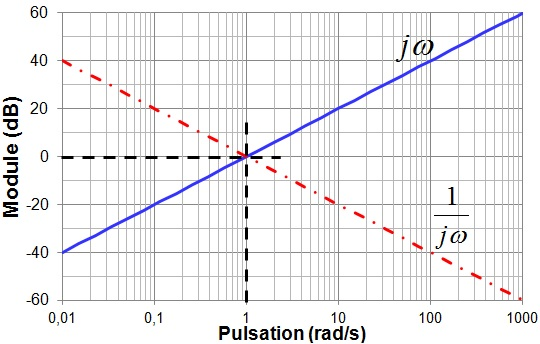
\includegraphics[scale=0.6]{images/Trace_asympt_jw.jpg}	
	\end{minipage}

	\vspace{1\baselineskip}
	
	\begin{minipage}[l]{0.5\linewidth}
		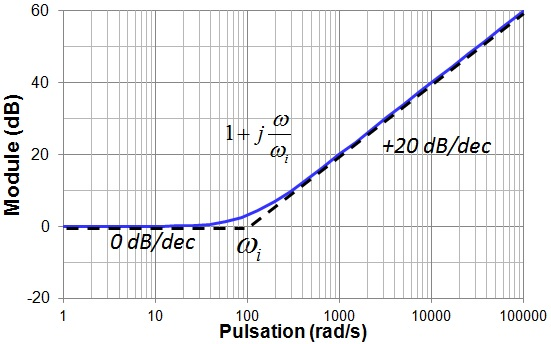
\includegraphics[scale=0.6]{images/Trace_asympt__1_plus_jw.jpg}
	\end{minipage} \hfill
	\begin{minipage}[c]{0.50\linewidth}
		Considérons maintenant le terme $1+j\frac{\omega}{\omega_{i}}$.	Tant que la pulsation est inférieure à $\omega_{i}$, le module reste constant, proche de 1 (soit 0 dB). Par contre, au-delà de $\omega_{i}$, le module augmente linéairement avec la fréquence, en +20 dB/dec. Entre ces deux comportements asymptotiques, l'évolution fréquentielle est plus compliquée à tracer précisément. Néanmoins, en ramenant le tracé à deux droites de pente 0 et +20 dB/dec se coupant en $\omega_{i}$, on obtient une représentation simplifiée mais montrant précisément la fréquence de coupure et les tendances asymptotiques de la fonction de transfert en dessous et au-dessus de la fréquence de coupure.	
	\end{minipage}

	\begin{minipage}[l]{0.5\linewidth}
		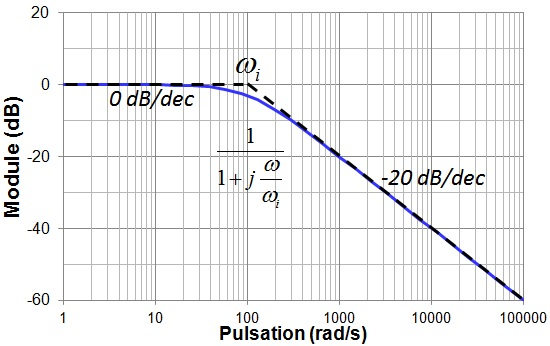
\includegraphics[scale=0.6]{images/Trace_asympt__1_moins_jw.jpg}
	\end{minipage} \hfill
	\begin{minipage}[c]{0.50\linewidth}
		De même, on peut représenter le tracé asymptotique du terme $\frac{1}{1+j\frac{\omega}{\omega_{i}}}$. Lors du passage en décibel, il devient : $20log(\frac{1}{1+j\frac{\omega}{\omega_{i}}}) = -20log(1+j\frac{\omega}{\omega_{i}})$. C'est donc le même terme que précédemment, mais au signe près. 	
	\end{minipage}
	
	\vspace{0.5\baselineskip}
	
	La phase de ces deux termes est égale à $+/-arctan(\frac{\omega}{\omega_{i}})$. On peut aussi en déduire deux comportements asymptotiques. Tant que la pulsation est largement inférieure à $\omega_{i}$, c'est la partie réelle qui domine donc la phase est proche de 0. Dès que la pulsation est bien plus grande que $\omega_{i}$, c'est la partie imaginaire et la phase tend vers $+/-\frac{\pi}{2}$. C'est ce qu'illustre la figure ci-dessous. On remarque le passage par $+/-\frac{\pi}{4}$ au passage par $\omega_{i}$.
	
	\begin{figure}[h!]
		\centering
		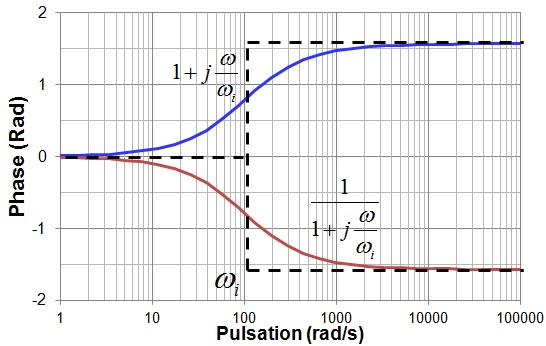
\includegraphics[scale=0.6]{images/Trace_asympt_phase_1_plus_jw.jpg}
	\end{figure}

	La multiplication des termes précédents par une constante réelle G, dans un diagramme de Bode en échelle log-log, introduit un simple décalage vertical du tracé égal à 20log(G) sans introduire de déphasage supplémentaire.
		
	\begin{minipage}[l]{0.5\linewidth}
		Il est possible qu'une racine soit multiple. Si elle apparait k fois, on verra un terme du type $(1+j\frac{\omega}{\omega_{i}})^{k}$ dans la fonction de transfert. Le passage en décibel de ce terme donne : $20log((1+j\frac{\omega}{\omega_{i}})^{k})=20k\cdot log(1+j\frac{\omega}{\omega_{i}})$. On retrouve donc le même genre de tracé asymptotique qu'au-dessus, mais le rythme de croissance (ou de décroissance) du module au-dessus de la fréquence de coupure est de +20xk dB/dec. Dans le cas d'une racine double, la pente sera de 40 dB/dec; 60 dB/dec pour une racine triple ... Dans l'exemple ci-contre, on considère une racine double. Ci-dessous, la phase de ce terme est tracé. Comme précédemment, on observe deux tendances asymptotiques : une phase tendant vers 0 en-dessous de $\omega_{i}$, puis une phase tendant vers $pi$ au-dessus de $\omega_{i}$. Dans le cas où la racine apparaît k fois, le déphasage tendra vers $k \cdot \frac{\pi}{2}$.	
	\end{minipage} \hfill
	\begin{minipage}[c]{0.50\linewidth}
		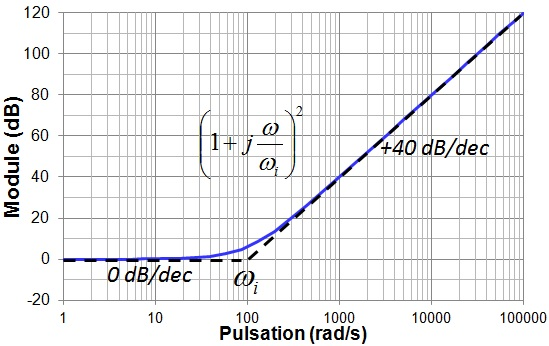
\includegraphics[scale=0.6]{images/Trace_asympt__1_plus_jw_carre.jpg}	
	\end{minipage}
	
	\vspace{1\baselineskip}
	
	\begin{figure}[h!]
		\centering
		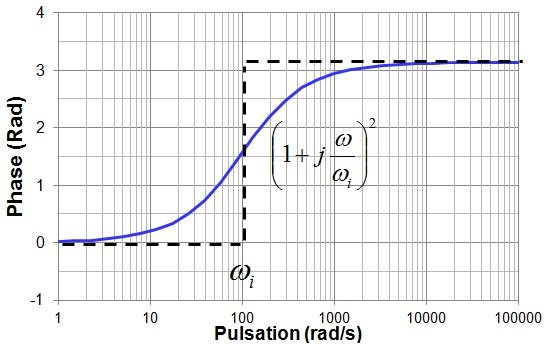
\includegraphics[scale=0.6]{images/Trace_asympt_phase_1_plus_jw_carre.jpg}
	\end{figure}
	
	Nous n'avons considéré que des cas particuliers de fonctions de transfert relativement simple. Comment faire lorsque l'expression de la fonction de transfert présente plusieurs termes au numérateur et au dénominateur. Là encore, le tracé dans un graphe log-log simplifie grandement les choses. Pour le tracé du module, après un passage en décibel, l'équation \ref{TF_usuelle_filtre} peut s'écrire sous la forme suivante. On retrouve les termes élémentaires vus précédemment. Le tracé asymptotique de cette fonction de transfert ne sera que l'addition des tracés asymptotiques individuels de chaque terme élémentaire. Si sur une plage de fréquence, deux termes ont une pente donnée, le comportement asymptotique résultant sera la somme de ces pentes. 
	
	\begin{equation}\label{}
	20log(H(\omega))=20log(G\frac{\prod_{i=1}^{m}(1+j\frac{\omega}{\omega_{i}})}{\prod_{j=1}^{n}(1+j\frac{\omega}{\omega_{j}})})=20log(G)+\sum_{i=1}^{m}20log(1+j\frac{\omega}{\omega_{i}})-\sum_{j=1}^{n}20log(1+j\frac{\omega}{\omega_{j}})
	\end{equation}
	
	De la même manière, la phase de la fonction de transfert sera obtenue en additionnant les déphasages introduits par chacun des termes élémentaires, comme le montre l'équation ci-dessous.
	\begin{equation}\label{key}
	arctan(H(\omega))=\sum_{i=1}^{m}arctan(\frac{\omega}{\omega_{i}})-\sum_{j=1}^{n}arctan(\frac{\omega}{\omega_{j}})
	\end{equation}
	
	Nous allons illustrer comment réaliser cette opération à travers un exemple. Considérons la fonction de transfert suivante :
	\begin{equation*}
	H(\omega) = 2\frac{j\omega(1+j\frac{\omega}{1000})}{1+j\frac{\omega}{10}}
	\end{equation*}
	
	
	La fonction de transfert est déjà mise sous une forme équivalente à l'équation \ref{TF_usuelle_filtre}. On identifie trois termes :
	\begin{enumerate}
		\item $2j\omega$
		\item $1+j\frac{\omega}{1000}=1+j\frac{\omega}{\omega_{2}}$
		\item $1+j\frac{\omega}{10}=1+j\frac{\omega}{\omega_{1}}$\\
	\end{enumerate}
	
	 On trace individuellement le comportement asymptotique de chaque terme. On commence par le tracé du module. Sur la figure \ref{Fig:Construction_trace_asympt_module}, le comportement asymptotique des trois termes est représenté. On repère les deux fréquences de transition $\omega_{1}$ et $\omega_{2}$. Sur les trois plages de fréquence ainsi délimitées, on additionne les morceaux des tracés asymptotiques. Entre $\omega_{1}$ et $\omega_{2}$, l'augmentation en 20 dB/dec du module liée au terme 1 est compensée par la décroissance due au terme 2. Le coefficient multiplicateur 2 conduit à un décalage de +6 dB du module.
	 
	 De la même manière, on réalise le tracé asymptotique de la phase. Le terme 1 introduit un déphasage constant de $\frac{\pi}{2}$. Le déphasage du terme 2 tend vers $\frac{\pi}{2}$ à l'infini, tandis que celui du terme 3 tend vers $-\frac{\pi}{2}$. Le résultat de la construction est présenté sur la figure \ref{Fig:Construction_trace_asympt_phase}.
	 
	 \begin{figure}[h!]
	 	\centering
	 	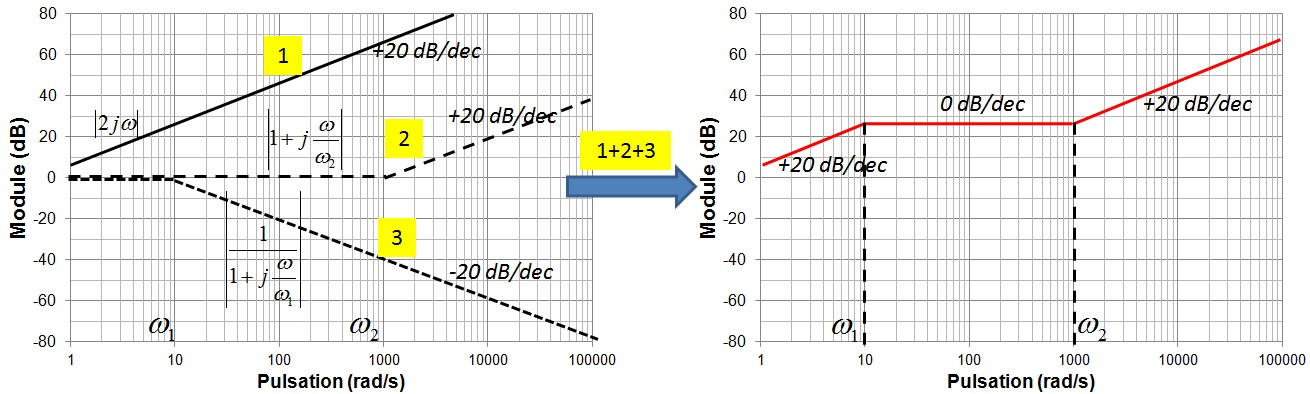
\includegraphics[scale=0.5]{images/Constr_trace_asympt_Module.jpg}
	 	\caption{Construction du tracé asymptotique du module de la fonction de transfert exemple}	
	 	\label{Fig:Construction_trace_asympt_module} 
	 \end{figure}
 
 	\begin{figure}[h!]
 		\centering
 		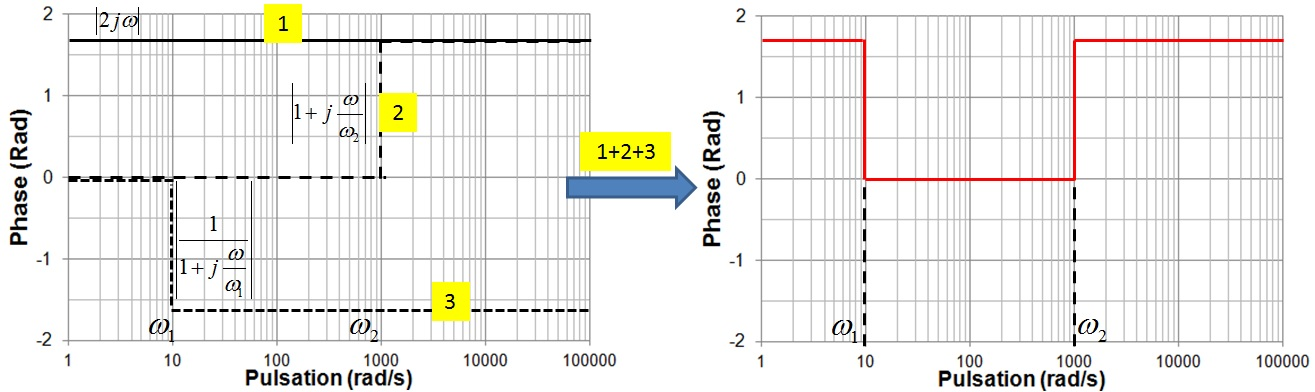
\includegraphics[scale=0.5]{images/Constr_trace_asympt_Phase.jpg}
 		\caption{Construction du tracé asymptotique de la phase de la fonction de transfert exemple}	
 		\label{Fig:Construction_trace_asympt_phase} 
 	\end{figure}
 
 	A titre de comparaison, le module et la phase de cette fonction de transfert sont tracés sur un diagramme de Bode. On vérifie que les tracés asymptotiques reflètent correctement les tendances du module et de la phase de la fonction de transfert.
 	
 	\begin{figure}[h!]
 		\centering
 		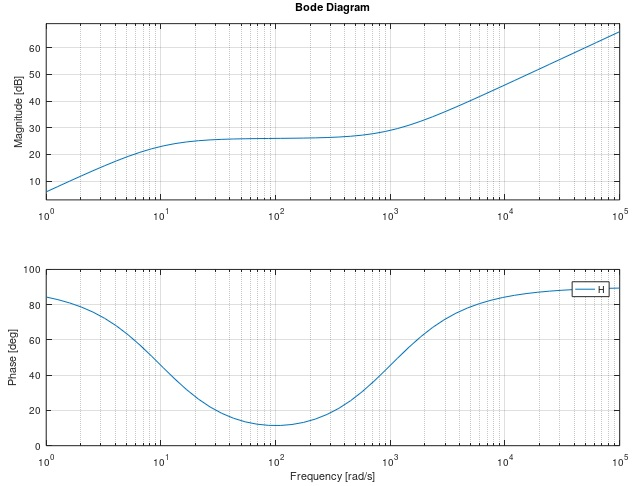
\includegraphics[scale=0.7]{images/Diag_Bode_Exemple_Octave.jpg}
 		\caption{Diagramme de Bode de la fonction de transfert exemple}	
 		\label{Fig:Diag_Bode_TF_exemple} 
 	\end{figure}
 
 	
	\vspace{1\baselineskip}


	\section{Les principales caractéristiques d'un filtre}
	Lorsqu'on analyse un filtre ou lorsqu'on cherche à le dimensionner, plusieurs caractéristiques sont étudiées. Celles-ci définissent le comportement fréquentiel global. Nous allons les définir ici. 
	
	\subsection{Gain}
	
	Le gain est le module de la fonction de transfert et varie donc avec la fréquence. Néanmoins, on peut spécifier une valeur unique, qui correspond généralement à la valeur maximale du gain.
	
	\subsection{Fréquence(s) de coupure}
	
	Elles correspondent aux fréquences auxquelles le gain présente un changement de tendance. Dans la pratique, on considère un critère d'atténuation du gain de -3 dB (soit une division du gain par $\sqrt{2}$). On appelle fréquence de coupure (en toute rigueur fréquence de coupure à -3dB) d’un filtre toute fréquence positive ou nulle $f_{c}$ vérifiant :
	
	\begin{equation}\label{key}
	|H(f_{c})|=\frac{\underset{\forall f \in \mathbb{R}^{+}}{max}(|H(f)|)}{\sqrt{2}} \Rightarrow~G_{dB}(f_{c})=\underset{\forall f \in \mathbb{R}^{+}}{max}(G_{dB}(f))-3
	\end{equation}
	Tout filtre admet alors une ou plusieurs fréquences de coupures : un filtre de gabarit passe-bas ou de gabarit passe-haut n’a qu’une fréquence de coupure, tandis qu’un filtre passe-bande ou coupe-bande classique a deux fréquences de coupure.
	
	\subsection{Bande passante}
	
	La sélectivité du filtre est donnée par sa bande passante. Il s'agit de la plage de fréquence sur laquelle l'atténuation apportée par le filtre est faible. Elle est délimitée par deux fréquences, définies selon un critère d'atténuation par rapport au gain maximal obtenu dans la bande passante. Un critère courant consiste à considérer une atténuation de -3 dB. La bande passante est donc la bande de fréquence où le gain reste compris entre sa valeur maximale et sa valeur maximale atténuée de 3 dB. On définit la bande passante d’un filtre comme l’ensemble des fréquences f de $\mathbb{R}^{+}$ pour lesquelles le module de la fonction de transfert demeure au moins égal à $\frac{1}{\sqrt{2}}$ fois sa valeur maximale. 
	La bande passante spécifie donc le domaine de fréquences à l’intérieur duquel le gain du filtre demeure plus ou moins constant, ou du moins ne chute pas de plus de 3 dB. Elle donne ainsi la plage de fréquences que le filtre va laisser passer, d’où son nom de bande passante ! 
	
	La bande passante d’un filtre est constituée d’un ou plusieurs intervalles de $\mathbb{R}^{+}$, les bornes de ces intervalles étant données par les fréquences de coupure du filtre. Par exemple, la bande passante d’un filtre passe-bas est de la forme [0; fc] où fc est l’unique fréquence de coupure, tandis que la bande passante d’un filtre passe-haut est de la forme [fc;$+\infty$] ; la bande passante d’un filtre passe-bande classique (i.e. avec une seule bande passante) est de la forme $[f_{c1}; f_{c2}]$ où $f_{c1}$ et $f_{c2}$ sont les deux fréquences de coupure, tandis que la bande passante d’un filtre coupe-bande classique (i.e. avec une seule bande coupée) est de la forme $[0;f_{c1}]$ + $[f_{c2};+\infty]$.
	
	\subsection{Ordre du filtre}
	L'ordre du filtre est lié au nombre de pôles de sa fonction de transfert. Il conditionne la pente de la variation du gain en dehors de la bande passante. Si l'ordre du filtre est égal à n, la pente évolue en $+/-20\cdot n~dB/dec$.
	
	\subsection{Fréquences de résonance et d'antirésonance}
	Lorsque les filtres présentent des racines complexes, elles sont généralement doubles et conjuguées.	Prenons l'exemple d'un filtre présentant deux pôles complexes et conjuguées $p_{0}$ et $p_{0}^{*}$, où $p_{0}=\alpha+j\omega_{0}$.
	\begin{equation*}
	H(p)=\frac{1}{(p+p_{0})p+p_{0})^{*}}=\frac{1}{(p+\alpha)^{2}+(\omega_{0})^{2}}
	\end{equation*}
	
	Supposons que la partie réelle $\alpha$ des racines est faible et plaçons nous en régime harmonique. La fonction de transfert est donnée par :
	\begin{equation*}
	H(\omega)=\frac{1}{(j\omega+\alpha)^{2}+(\omega_{0})^{2}}
	\end{equation*}
	Si on excite le filtre à une pulsation proche de $\omega_{0}$, alors le dénominateur tend vers 0, faisant croître fortement le module de la fonction de transfert autour de $\omega_{0}$. On assiste à un phénomène de résonance. La fréquence $f_{0}=\frac{\omega_{0}}{2\pi}$ est appelée fréquence de résonance. Si on excite un filtre par un signal (co)sinusoïdal à cette fréquence, le signal de sortie sera affectée par une forte oscillation.
	
	Inversement, si la fonction de transfert présente deux zéros complexes et conjuguées, le module tendra vers 0 autour de $\omega_{0}$. On parlera de phénomène d'antirésonance, autour d'une fréquence dite d'antirésonance. Un filtre aura tendance à éliminer efficacement un signal (co)sinusoïdal à cette fréquence.
	
	\vspace{1\baselineskip}
	
	
	\section{Les différents types de filtres}
	On classifie les filtres en quatre types selon leur sélectivité fréquentielle : 
	\begin{itemize}
		\item un filtre passe-bas laisse passer les basses fréquences et atténue les hautes fréquences
		\item un filtre passe-haut laisse passer les hautes fréquences et atténue les basses fréquences
		\item un filtre passe-bande ne laisse passer que les fréquences contenues dans un intervalle donné
		\item un filtre coupe-bande n'atténue  que les fréquences contenues dans un intervalle donné
	\end{itemize}

	Dans cette partie, nous allons rapidement passer en revue les expressions et les caractéristiques de ces différents filtres, pour les ordres 1 et 2. Nous tracerons aussi leur diagramme de Bode.
	
	
	\subsection{Filtre passe-bas d'ordre 1}
	L'expression général de la fonction de transfert d'un filtre passe-bas d'ordre 1 est donnée par l'équation \ref{FT_passe_bas_1}, où $f_{c}$ est la fréquence de coupure. Au-dessus de cette fréquence, le filtre apporte une atténuation augmentant en 20 dB/dec. A la fréquence de coupure, le gain est égal à $\frac{1}{\sqrt{2}}$ d'où une atténuation de 3 dB. Le tracé dans le diagramme de Bode est présenté à la figure \ref{Fig:Bode_passe_bas_1}.
	
	\begin{equation}\label{FT_passe_bas_1}
	H(f) = \frac{1}{1+j\frac{f}{f_{c}}}
	\end{equation}
	
	\begin{figure}[h!]
		\centering
		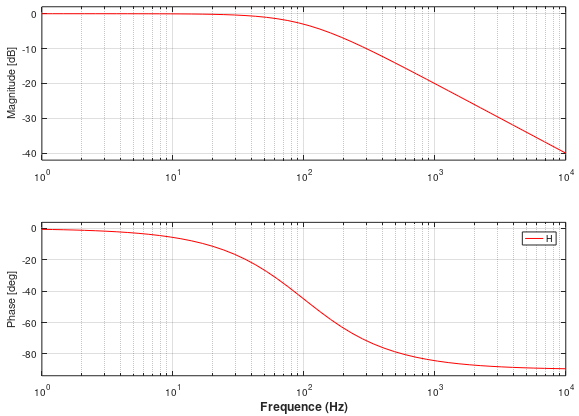
\includegraphics[scale=0.7]{images/Bode_passe_bas_1.png}
		\caption{Diagramme de Bode d'un filtre passe-bas d'ordre 1 ($f_{c}=100 Hz$)}	
		\label{Fig:Bode_passe_bas_1} 
	\end{figure}


	\subsection{Filtre passe-haut d'ordre 1}
	L'expression générale de la fonction de transfert d'un filtre passe-haut d'ordre 1 est donnée par l'équation \ref{FT_passe_haut_1}, où $f_{c}$ est la fréquence de coupure. En dessous de cette fréquence, le filtre apporte une atténuation diminuant en 20 dB/dec. A la fréquence de coupure, le gain est égal à $\frac{1}{\sqrt{2}}$ d'où une atténuation de 3 dB. Le tracé dans le diagramme de Bode est présenté à la figure \ref{Fig:Bode_passe_haut_1}.
	
	\begin{equation}\label{FT_passe_haut_1}
	H(f) = \frac{j\frac{f}{f_{c}}}{1+j\frac{f}{f_{c}}}
	\end{equation}
	
	\begin{figure}[h!]
		\centering
		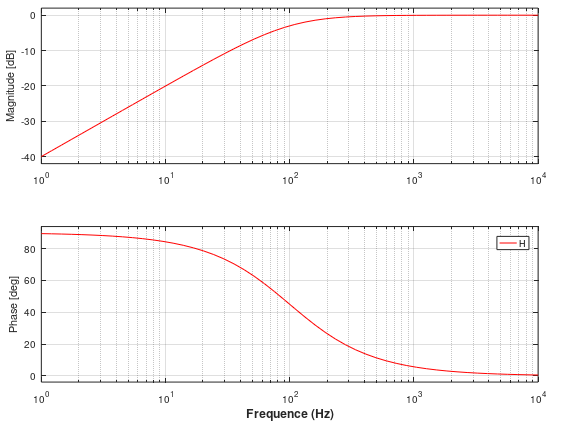
\includegraphics[scale=0.7]{images/Bode_passe_haut_1.png}
		\caption{Diagramme de Bode d'un filtre passe-haut d'ordre 1 ($f_{c}=100 Hz$)}	
		\label{Fig:Bode_passe_haut_1} 
	\end{figure}

	
	\subsection{Filtre passe-bas d'ordre 2}
	
	L'expression générale de la fonction de transfert d'un filtre passe-bas d'ordre 2 est donnée par l'équation \ref{FT_passe_bas_2}, où $f_{c}$ est la fréquence de coupure et $\zeta$ le coefficient d'amortissement. Au-dessus de cette fréquence, le filtre apporte une atténuation augmentant en 40 dB/dec. Selon la valeur du coefficient d'amortissement, on observe un accroissement du gain autour de la fréquence de coupure. Le tracé dans le diagramme de Bode est présenté à la figure \ref{Fig:Bode_passe_bas_1} pour deux valeurs du coefficient d'amortissement.
	
	
	\begin{equation}\label{FT_passe_bas_2}
	H(f) = \frac{1}{1+2\zeta j\frac{f}{f_{c}}+(j\frac{f}{f_{c}})^{2}}
	\end{equation}

	\begin{figure}[h!]
		\centering
		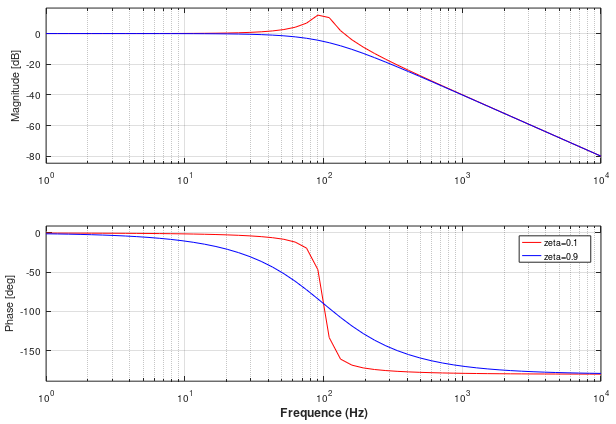
\includegraphics[scale=0.75]{images/Bode_passe_bas_2.png}
		\caption{Diagramme de Bode d'un filtre passe-bas d'ordre 2 ($f_{c}=100 Hz$)}	
		\label{Fig:Bode_passe_bas_2} 
	\end{figure}
	
	
	
	\subsection{Filtre passe-haut d'ordre 2}
	L'expression générale de la fonction de transfert d'un filtre passe-haut d'ordre 2 est donnée par l'équation \ref{FT_passe_haut_2}, où $f_{c}$ est la fréquence de coupure et $\zeta$ le coefficient d'amortissement. En dessous de cette fréquence, le filtre apporte une atténuation diminuant en 40 dB/dec. Selon la valeur du coefficient d'amortissement, on observe un accroissement du gain autour de la fréquence de coupure. Le tracé dans le diagramme de Bode est présenté à la figure \ref{Fig:Bode_passe_haut_2} pour deux valeurs du coefficient d'amortissement.
	
	\begin{equation}\label{FT_passe_haut_2}
	H(f) = \frac{(\frac{f}{f_{c}})^{2}}{1+2\zeta j\frac{f}{f_{c}}+(j\frac{f}{f_{c}})^{2}}
	\end{equation}
	
	\begin{figure}[h!]
		\centering
		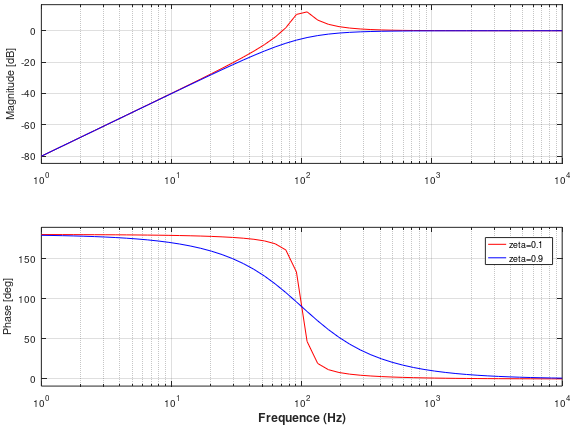
\includegraphics[scale=0.75]{images/Bode_passe_haut_2.png}
		\caption{Diagramme de Bode d'un filtre passe-haut d'ordre 2 ($f_{c}=100 Hz$)}	
		\label{Fig:Bode_passe_haut_2} 
	\end{figure}
	
	\subsection{Filtre passe-bande d'ordre 2}
	L'expression générale de la fonction de transfert d'un filtre passe-bande d'ordre 2 est donnée par l'équation \ref{FT_passe_bande}, où $f_{c}$ est la fréquence de résonance ou fréquence centrale et $\zeta$ le coefficient d'amortissement. Il n'existe pas de filtre passe-bande d'ordre 1. Le filtre atténue toutes les fréquences de part et d'autre de la fréquence de résonance, avec une pente en 40 dB/dec. Selon la valeur du coefficient d'amortissement, le gain est plus ou moins important dans la bande passante. Cependant, plus l'amortissement est élevé, plus la bande passante s'élargit. Le tracé dans le diagramme de Bode est présenté à la figure \ref{Fig:Bode_passe_bande} pour deux valeurs du coefficient d'amortissement.
	
	\begin{equation}\label{FT_passe_bande}
	H(f) = \frac{(j\frac{f}{f_{c}})^{2}}{1+2\zeta j\frac{f}{f_{c}}+(j\frac{f}{f_{c}})^{2}}
	\end{equation}
	
	On appelle $Q = \frac{1}{2\zeta}$ le facteur de qualité. La bande passante de ce filtre est donnée par $\Delta f=\frac{f_{c}}{Q}$.
	
	\begin{figure}[h!]
		\centering
		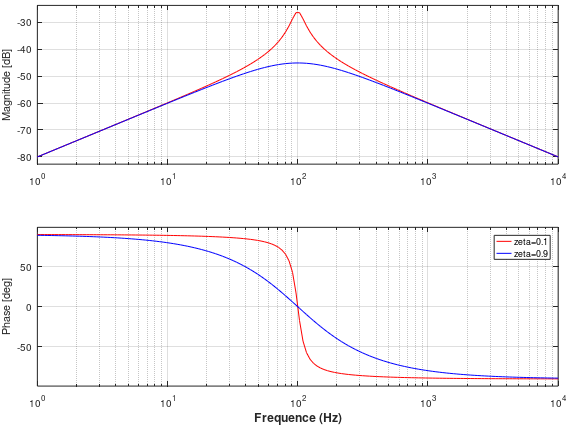
\includegraphics[scale=0.75]{images/Bode_passe_bande.png}
		\caption{Diagramme de Bode d'un filtre passe-bande d'ordre 2 ($f_{c}=100 Hz$)}	
		\label{Fig:Bode_passe_bande} 
	\end{figure}
	
	\subsection{Filtre coupe-bande d'ordre 2}
	L'expression générale de la fonction de transfert d'un filtre coupe-bande d'ordre 2 est donnée par l'équation \ref{FT_coupe_bande}, où $f_{c}$ est la fréquence d'antirésonance ou fréquence centrale et $\zeta$ le coefficient d'amortissement. Il n'existe pas de filtre coupe-bande d'ordre 1. Le filtre laisse passer toutes les fréquences de part et d'autre de la fréquence centrale. La capacité du filtre à couper une bande de fréquence est liée au coefficient d'amortissementt.
	
	\begin{equation}\label{FT_coupe_bande}
	H(jf) = \frac{1+(j\frac{f}{f_{c}})^{2}}{1+2\zeta j\frac{f}{f_{c}}+(j\frac{f}{f_{c}})^{2}}
	\end{equation}
	
	\begin{figure}[h!]
		\centering
		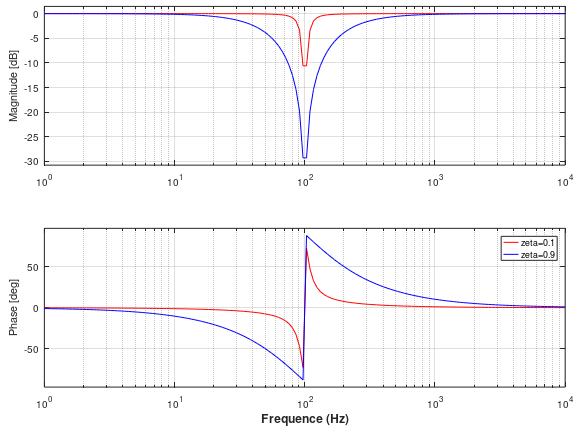
\includegraphics[scale=0.75]{images/Bode_coupe_bande.png}
		\caption{Diagramme de Bode d'un filtre coupe-bande d'ordre 2 ($f_{c}=100 Hz$)}	
		\label{Fig:Bode_coupe_bande} 
	\end{figure}
	
	\subsection{Mise en cascade filtre}
	
	Pour augmenter la sélectivité des filtres, il est nécessaire d'accroître leur ordre. On se rend compte qu'on doit pouvoir créer des filtres d'ordre élevé à partir des filtres précédents en les chainant. Supposons que l'on mette en cascade N filtres comme le montre la figure \ref{Fig:Cascade_filtre}. En supposant que le chainage de ces filtres n'influe pas sur leurs caractéristiques, les signaux de sortie et d'entrée sont reliés entre eux par l'équation \ref{Cascade_filtre}.
	\begin{equation*}
	Y(f)=H_{N}(f)Y_{N-1}(f)=H_{N}(f)H_{N-1}(f)Y_{N-2}(f)=H_{N}(f)H_{N-1}(f)...H_{1}(f)X(f)
	\end{equation*}
	\begin{equation}\label{Cascade_filtre}
	Y(f)=X(f)\prod_{i=1}^{N}H_{i}(f)
	\end{equation}
	
	
	
	La condition précédente doit être vérifiée pour utiliser la relation \ref{Cascade_filtre}. Lorsqu'on réalise un filtre électronique, des conditions d'adaptation d'impédance sont requises pour garantir que le filtre en aval ne modifie pas la tension en sortie du filtre placée en amont. 
	
	
	\begin{figure}[h!]
		\centering
		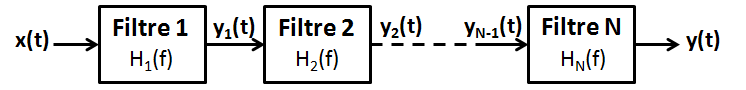
\includegraphics[scale=0.6]{images/Cascade_filtre.png}
		\caption{Mise en cascade de filtre}	
		\label{Fig:Cascade_filtre} 
	\end{figure}

	
	

	
	
	\section{Exercices }
	
	\subsubsection{Exercice 1}
	Soit les fonctions de transfert suivantes (en fonction de la fréquence). Esquissez le diagramme de Bode (asymptotique). \\
	
	a. $G(\omega)=\frac{j10\omega}{(1+j\frac{\omega}{628})(1+j\frac{\omega}{6280})(1+j\frac{\omega}{31400})}$\\
	
	b. $H(p)=\frac{p^3+4p^2+4p}{p^2+60p+800}$\\
	
	c. $Z(p)=\frac{p+10}{p(p+100)}$\\
	
	
	\subsubsection{Exercice 2 - Circuit bouchon}
	On considère le filtre décrit ci-dessous.
	
	\begin{figure}[h!]
		\centering
		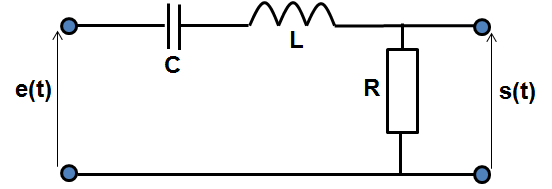
\includegraphics[scale=0.5]{images/circuit_bouchon.png} 
	\end{figure}
	
	1. Etablir la fonction de transfert $H(\omega)$ de ce filtre. On la mettra sous la forme : $H(\omega)=\frac{2\alpha \omega}{2\alpha \omega+j(\omega^{2}-\omega_{0}^{2})}$. Précisez la signification des termes $\alpha$ et $\omega_{0}$.\\
	
	2. Tracez 'évolution de la fonction de transfert de ce filtre en fonction de la fréquence. Précisez l'amplitude maximale et les fréquences caractéristiques. Quelle est la nature du filtre ? Son ordre ?\\
	
	3. Déterminez la bande passante à 3 dB de ce filtre. \\
	
	4. Déterminez le facteur de qualité de ce filtre. \\
	
	5. On fixe L = $100 \mu H$. On souhaite réaliser un filtre centré sur 200 kHz avec une bande passante de 10 kHz. Proposez des valeurs pour R et C.\\
	
	
	\subsubsection{Exercice 3}
	On considère le filtre passif ci-dessous. On utilisera les valeurs suivantes : R = 1 k$\Omega$ et C = 100 nF.
	
	\begin{figure}[h!]
		\centering
		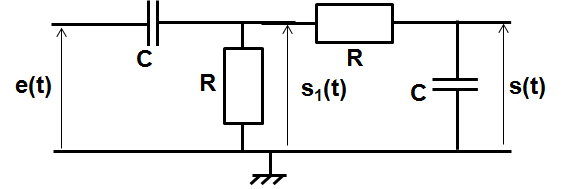
\includegraphics[scale=0.5]{images/Exo_4_3.png} 
	\end{figure}
	
	
	1. Déterminez l'expression de l'impédance formée par le circuit en aval du premier condensateur.\\
	
	2. En déduire la relation entre les tensions $e$ et $s_1$. En déduire la fonction de transfert du circuit.\\
	
	3. Quels sont les pôles et les zéros du filtre. \\
	
	4. Pour les valeurs de R et de C, tracez le diagramme asymptotique de Bode. Précisez les fréquences de coupure du filtre, ainsi que la nature du filtre.\\
	
	\subsubsection{Exercice 4}
	On dispose d'un filtre dont la fonction de transfert est donnée par $H(p)=\frac{1}{(p+2)^2}$.
	
	1. Tracez la réponse fréquentielle du filtre dans le diagramme de Bode. Quelle est la nature du filtre ? Quelle est sa fréquence de coupure ? \\
	
	2. Calculez sa réponse impulsionnelle.\\
	
	3. Calculez sa réponse indicielle. \\
	

	
	\subsubsection{Exercice 5 - Mise en cascade de filtres}
	On considère le filtre RC ci-dessous.
	
	\begin{figure}[h!]
		\centering
		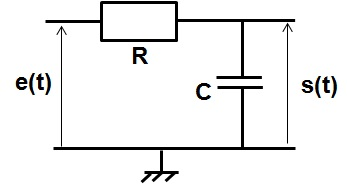
\includegraphics[scale=0.5]{images/Filtre_RC_passe_bas.jpg} 
	\end{figure}
	
	1. Calculez la fonction de transfert de ce filtre H(f).
	
	2. Précisez sa nature, sa fréquence de coupure, son ordre.
	
	3. On cascade deux filtres de ce type. Calculez sa fonction de transfert $H_{2}(f)$.
	
	4. Vérifie t-on $H_{2}(f)=H(f)^{2}$ ? Pourquoi ?
